
For the grid output, two hierarchic classes have been implemented - \textit{CurvilinearVTKWriter} and \textit{CurvilinearVTKGridWriter}. The former discretizes and accumulates entities and fields one-by-one and later writes them to a file, and the latter uses the former to write the entities of the grid by iterating over them. \textit{CurvilinearVTKWriter} supports VTK, VTU and PVTU file formats.  
In order to append an entity to the writer, one needs to call the following member function:

\begin{mybox}
\begin{lstlisting}
  template<int mydim, int subdim>
  void addCurvilinearElement(
	  const Dune::GeometryType & geomtype,
	  const GlobalCoordinateVec & nodeSet,
	  const TagVector & tagSet,
	  int elementOrder,
	  int nDiscretizationPoint,
	  bool interpolate,
	  bool explode)
\end{lstlisting}
\end{mybox}
\noindent
where

\begin{itemize}  
  \item \textit{mydim} is the dimension of the entity to be written
  \item \textit{subdim} is the dimension of the subentities into which the entity is to be discretized. For example, a tetrahedron can be discretized into smaller tetrahedra, or one can only write its faces, discretized into smaller triangles, or its edges discretized into smaller edges
  \item \textit{geomtype} is the geometry type of the entity. Currently only simplex entities are supported
  \item \textit{nodeSet} is a vector of global coordinates of interpolatory vertices of the entity in correct order \ref{impl-gmsh-numbering-convention}
  \item \textit{tagSet} is a set of 3 scalar fields used for diagnostics, which typically accompany all written elements. Namely, they are the physical tag, the partition type, and the containing process rank in that very order
  \item \textit{nDiscretizationPoint} is the number of vertices into which to discretize each edge. The number has to be at least 2
  \item \textit{interpolate} parameter determines how the virtual refinement of the entity is performed. If true, the regular grid of interpolatory points is re-used to subdivide the entity into smaller linear entities. If false, a new regular grid is constructed for this purpose, using the \textit{nDiscretizationPoint} parameter to determine the number of desired discretization vertices per edge. If the interpolation vertices are used the latter parameter is discarded. Note that the associated fields are sampled over the vertices of the virtual refinement grid, and thus increasing the virtual refinement is useful for better visualizing the element curvature and/or finer field resolution. Note that increasing \textit{nDiscretizationPoint} results in quadratic increase in both writing time and the resulting visualization file size, so the parameter must be used with care.
  \item \textit{explode} optional parameter shrinks all entities with respect to their mass-centers, allowing to better visualize the 3D structure of the grid. Default parameter is $0.0$, which corresponds to no shrinking, and the maximum allowed parameter is $0.99$
  %\item \textit{magnify} optional parameter expands all boundary surfaces with respect to the origin, allowing to better visualize the difference between boundary segments and element faces. By default there is no magnification
\end{itemize}


\begin{figure}
	\centering
	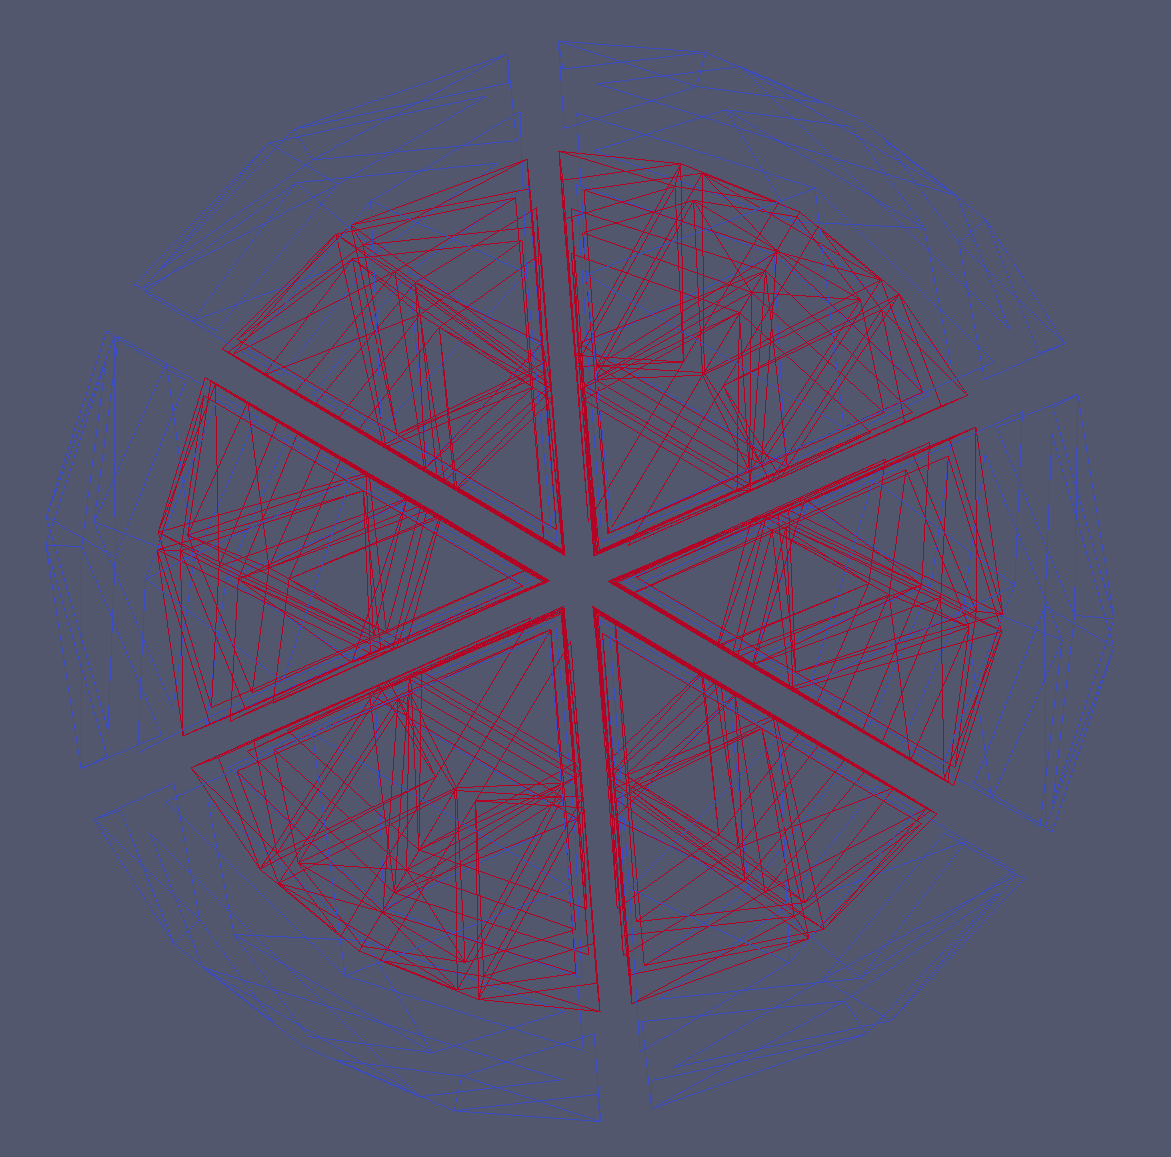
\includegraphics[scale=0.2]{images/gmshreader-vtk-wireframe}
	\caption{Visualization of an edge wireframe of a 32 element 2nd order mesh using the manual virtual refinement with  \textit{nDiscretizationPoint=3}  }
	\label{fig:gmshreader:wireframe}
\end{figure}

\noindent
By default, to write a grid to a PVTU file, one only needs to call the \textit{CurvilinearVTKGridWriter} write method

\begin{mybox}
\begin{lstlisting}
  void write(std::string path, std::string filenamePrefix)
\end{lstlisting}
\end{mybox}
\noindent
where \textit{path} is the output path, and \textit{filenamePrefix} is the desired file name without the extension. \textit{CurvilinearVTKGridWriter} is a flexible grid writing tool. By calling setup member functions, one can tune the following output
\begin{itemize}
 \item Set custom discretization order (\textit{nDiscretizationPoint} in the above)
 \item Determine individually, whether or not to write the entities of any of the following types: process boundaries, domain boundaries, interior boundaries, periodic boundaries, ghosts.
 \item An additional option (called PeriodicBind) allows to write lines connecting each pair of periodic faces, to visually check if the periodic grid is initialized correctly.
 \item Determine whether or not to write patience logging output
 \item Whether or not to reuse interpolation vertices (as explained above)
 \item Whether or not to use element explosion (as explained above)
 \item Whether to use ASCII or BINARY output format (currently only ASCII supported)
\end{itemize}

\noindent
In addition, the writer supports arbitrary number of scalar and vector fields, that can be written to the grid via the \textit{addFieldSet} routine. The fields must be provided in terms of functors, that return the field value given the entity, and the local coordinate. Currently, fields can be associated to elements and/or to faces. Currently the element fields are only wriiten over interior elements, and face fields are only written over Domain Boundaries and Interior Boundaries. \\

\noindent
For further details please consult the explanation of tutorials 3 and 4 \cref{usage-howto-tutorial-visualisation}, as well as the tutorial codes in the repository.


% \subsection{Optimal Sampling Rate}
% 
% Here we would like to discuss how many sampling points are required to represent the bounded curve using linear interpolation. This is necessary, for example, for visualisation. For a line segment, interpolating the curve bounded by 2 points, the analytic error is bounded by
% \begin{equation}
% 	\epsilon = |f(x) - g(x)| \leq \frac{1}{8} \max_{z \in [x_a, x_b]} \{ g''(z)  \} (x_a - x_b)^2
% \end{equation}
% \noindent
% where $f(x)$ is the line segment, $g(x)$ is the original function. $x_a$ and $x_b$ are arguments of the endpoints of the interval. \\
% 
% \noindent
% Given a large interval $L$ which we split into $N$ equal segments such that $x_b - x_a = L/N$, the maximal error over all interpolated intervals is bounded by
% \begin{equation}
% 	\epsilon_{\max} \leq \frac{L^2}{8 N^2} \max_{z \in L} \{ g''(z) \}
% \end{equation}
% \noindent
% This can be rewritten to obtain the necessary interval number per edge
% \begin{equation}
% 	N = \biggl \lceil \alpha \sqrt{ \max_{z \in L} \{ g''(z) \} } \biggr \rceil
% \end{equation}
% \noindent
% where $\alpha$ depends on precision and length of the interval. We observe that there is a problem with this formula, namely that if $g''(z) = 0$ we get 0 intervals, and if $g''(z)$ is small, we get 1 interval, and we would like 2, because there is at least some curvature, and it should be emphasized that the case is different from just straight line. Therefore we empirically modify the formula
% \begin{equation}
% 	N = \biggl \lceil \alpha \sqrt{ \max_{z \in L} \{ g''(z) \} } + 1 \biggr \rceil
% \end{equation}
% 
% \noindent
% Finally, since this equation is not exactly accurate for surfaces, and it is rather hard to make sense of optimal relative error, it is much easier to choose $\alpha$ empirically. We will generally operate with unit length edges ($L = 1$), and would like to, for example, have 5 points per edge with standard quadratic curvature $g(x) = x^2$. We obtain that $\alpha \approx 2.8$. \\
% 
% \noindent
% As a rule of thumb, we can calculate the expected number of intervals for a standard function $g(x) = \sum_i x^i$ using this formula. The first 5 orders will produce edge intervals $\{ 1, 5, 9, 17, 35\}$, which will correspond to the number of vertices per edge $\{ 2, 6, 10, 18, 36\}$, and thus the number of surface vertices ($i(i+1)/2$) will be given by $\{3, 21, 55, 171, 666\}$.